\documentclass[border=3pt]{standalone}
\usepackage{fontspec}
\setmainfont{Times New Roman}
\usepackage{pgfplots}
\pgfplotsset{compat=1.18}
\usetikzlibrary{arrows.meta,calc,positioning,shapes.geometric}
\definecolor{forest}{HTML}{346E57}
\definecolor{sage}{HTML}{E8EFEA}
\definecolor{clay}{HTML}{B77E60}
\definecolor{gray}{HTML}{718078}
\definecolor{rule}{HTML}{B7C3BA}
\definecolor{ink}{HTML}{000000}
\begin{document}
\hyphenpenalty=10000\exhyphenpenalty=10000
\fontsize{10}{12}\selectfont
\renewcommand{\small}{\fontsize{9}{11}\selectfont}
\renewcommand{\scriptsize}{\fontsize{8}{10}\selectfont}
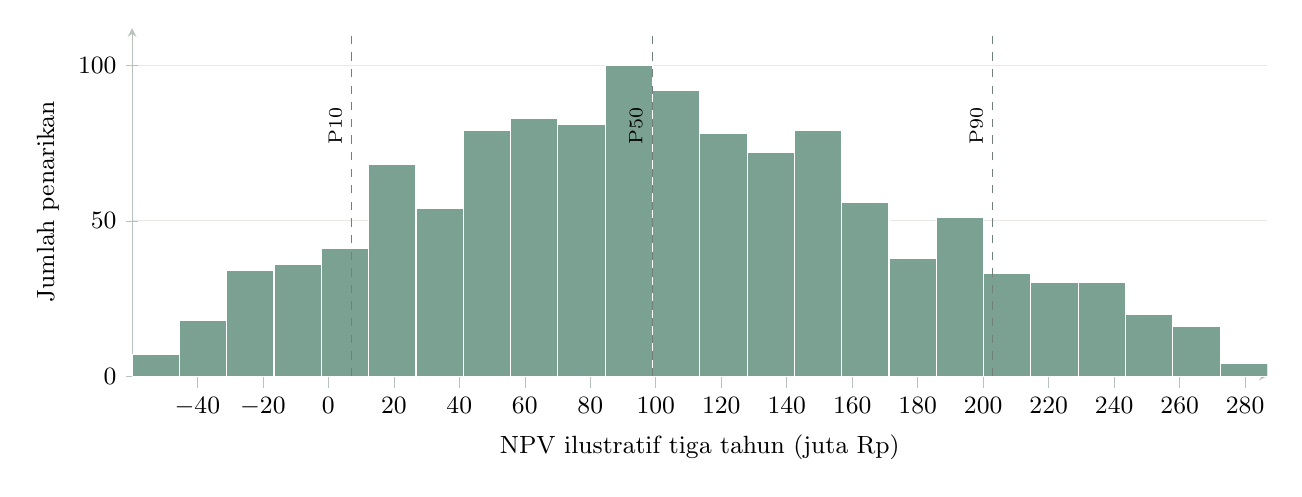
\begin{tikzpicture}\begin{axis}[width=16cm,height=6cm,scale only axis=false,
axis lines=left,axis line style={draw=rule},tick style={draw=rule},
tick label style={font=\small},label style={font=\small},
grid=major,grid style={draw=rule!35,line width=.3pt},
legend style={draw=none,fill=none,font=\small,at={(.5,-.26)},anchor=north},legend columns=-1,
ybar,bar width=14.4468,xlabel={NPV ilustratif tiga tahun (juta Rp)},ylabel={Jumlah penarikan},ymin=0,ymajorgrids=true,xmajorgrids=false,]
\addplot+[ybar interval,mark=none,fill=forest!65,draw=white] coordinates {(-59.918,7) (-45.4712,18) (-31.0243,34) (-16.5775,36) (-2.13067,41) (12.3162,68) (26.763,54) (41.2098,79) (55.6567,83) (70.1035,81) (84.5503,100) (98.9972,92) (113.444,78) (127.891,72) (142.338,79) (156.784,56) (171.231,38) (185.678,51) (200.125,33) (214.572,30) (229.019,30) (243.465,20) (257.912,16) (272.359,4) (286.806,0)};
\addplot[sharp plot,gray,dashed,forget plot] coordinates {(7.153600000000002,0)(7.153600000000002,112.00000000000001)};
\node[anchor=south,rotate=90,font=\scriptsize] at (axis cs:7.153600000000002,80.64) {P10};
\addplot[sharp plot,gray,dashed,forget plot] coordinates {(98.87899999999999,0)(98.87899999999999,112.00000000000001)};
\node[anchor=south,rotate=90,font=\scriptsize] at (axis cs:98.87899999999999,80.64) {P50};
\addplot[sharp plot,gray,dashed,forget plot] coordinates {(202.91379999999987,0)(202.91379999999987,112.00000000000001)};
\node[anchor=south,rotate=90,font=\scriptsize] at (axis cs:202.91379999999987,80.64) {P90};
\end{axis}\end{tikzpicture}
\end{document}
